\documentclass[12pt]{article}
\usepackage{graphicx}
\usepackage{amsmath}
\usepackage{mathtools}
\usepackage{gensymb}

\newcommand{\mydet}[1]{\ensuremath{\begin{vmatrix}#1\end{vmatrix}}}
\providecommand{\brak}[1]{\ensuremath{\left(#1\right)}}
\providecommand{\norm}[1]{\left\lVert#1\right\rVert}
\newcommand{\solution}{\noindent \textbf{Solution: }}
\newcommand{\myvec}[1]{\ensuremath{\begin{pmatrix}#1\end{pmatrix}}}
\let\vec\mathbf

\begin{document}
\begin{center}
\textbf\large{CHAPTER-7 \\ COORDINATE GEOMETRY}
\end{center}
\section*{Excercise 7.2}

Q2. Find a relation between x and y if the points $\vec(x, y), \vec(1, 2) \text{ and } \vec(7, 0)$ are collinear.
\\
\solution
\\
The coordinates are given as
	\begin{align}
	\vec{A} = \myvec{
		x\\
		y\\
		},
	\vec{B} = \myvec{
		1\\
		2\\
		},
	\vec{C} = \myvec{
		7\\
		0\\
		}
	\end{align}
For collinear, ar(ABC) should be equal to zero
	\begin{align}
		ar(ABC)&=\frac{1}{2}{\norm{\vec(\vec{A}-\vec{B})\times\vec(\vec{A}-\vec{C})}}=0\\
		\vec{A}-\vec{B} &=  \myvec{
  x \\
  y \\
 } - \myvec{
  1 \\
  2 \\
 } = \myvec{
 x-1 \\
 y-2 \\
 }
 \\
		\vec{A}-\vec{C} &=  \myvec{
  x \\
  y \\
 } - \myvec{
  7 \\
  0 \\
 } = \myvec{
 x-7 \\
 y \\
 }
 \\
		&=\frac{1}{2}\mydet{x-1 & x-7\\y-2 & y}=0\\
		&\implies x+3y-7=0
	\end{align}
	Suppose, if x=-2,y=3 , then area of triangle ABC is equal to zero which is collinear as shown in Figure:\ref{fig:Fig}
\begin{figure}[!h]
	\begin{center} 
	    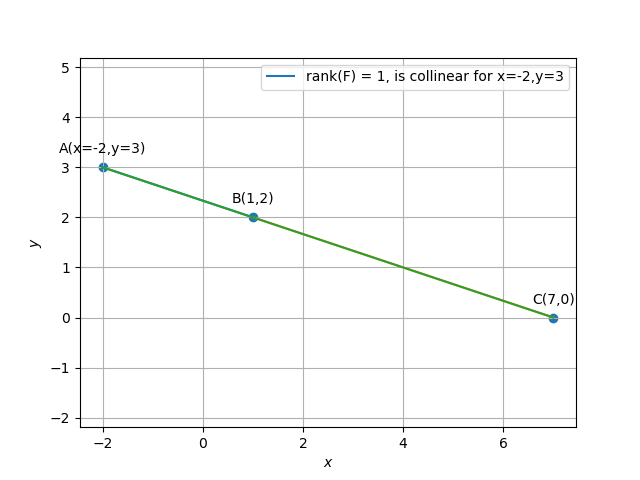
\includegraphics[width=\columnwidth]{./figs/sc1.png}
	\end{center}
\caption{}
\label{fig:Fig}
\end{figure}
\end{document}
